%==============================================================================
%  Robots.txt crawler-access restrictions and filing-window liquidity
%  Built 2026-06-15 from the current rerun (v2_all_search; abnormal Amihud
%  [-1,+1] vs [-60,-10]; TWFE + Borusyak et al. (2024)). NUMBERS: paper_table_stats.csv,
%  paper_summary_stats.csv, paper_hr_stats.csv, and the verified rev4 mechanism
%  draft. Do NOT reuse the superseded search16/[0,+5]/+13.2 numbers.
%
%  COMPILE: pdflatex -> bibtex -> pdflatex x2  (uses newtxtext = Times).
%  For LITERAL Times New Roman / Arial system fonts, compile with XeLaTeX and
%  replace the font block with:
%     \usepackage{fontspec}\setmainfont{Times New Roman}   % (Arial: \setmainfont{Arial})
%==============================================================================
\documentclass[12pt]{article}

\usepackage[a4paper,top=1in,bottom=1in,left=1.25in,right=1.25in]{geometry}
\usepackage{amsmath,amssymb}       % load BEFORE newtxmath
\usepackage{newtxtext,newtxmath}   % Times-equivalent body + math, 12pt
\usepackage{setspace}
\usepackage{booktabs,threeparttable,tabularx,multirow,array,makecell}
\usepackage{graphicx}
\usepackage{caption}
\usepackage[round]{natbib}
\usepackage[hidelinks]{hyperref}
\graphicspath{{figs/}}
\onehalfspacing                    % switch to \doublespacing for review copies
\pagenumbering{arabic}

\title{Robots.txt Crawler-Access Restrictions and the Liquidity of Disclosure Windows}
\author{Xueyang Liu\thanks{Universitat Ram\'on Llull. Preliminary draft; please do not circulate.}}
\date{\today}

\begin{document}
\maketitle

\begin{abstract}
\noindent We study what happens to stock liquidity around mandatory disclosures when a firm restricts automated access to its website through its \texttt{robots.txt} file. Using a staggered difference-in-differences design over 2021--2025, we find that firms that block search and discovery crawlers experience a rise in abnormal filing-window Amihud illiquidity in the $[-1,+1]$ trading-day window around 10-K and 10-Q filings, measured relative to a local pre-filing benchmark. The increase does not reflect lower trading participation or wider posted spreads; instead, filing-window price impact rises relative to the firm's local pre-filing benchmark---a stronger return-variance response with no decline in volume---the signature of a price-impact (market-depth) channel rather than a transaction-cost or participation channel. The effect concentrates among younger firms and is accompanied, among firms with pre-existing analyst coverage, by suggestive evidence of greater analyst engagement. We find no evidence that the effect operates through delayed price incorporation, posted-spread widening, EDGAR substitution, or that it is specific to AI/LLM crawlers. The evidence is consistent with a depth / price-impact (Kyle, 1985) interpretation rather than a single identified channel.
\end{abstract}

%==============================================================================
\section{Introduction}\label{sec:intro}
%==============================================================================
A mandatory disclosure is useful to investors only if they can find it. For most of the history of securities regulation, finding it meant a person reading a filing; increasingly, it means a machine retrieving one. Search engines, answer engines, and the data vendors that resell their indexes now sit between a firm's disclosures and the investors who trade on them, and they reach a firm's investor-relations pages, filing links, and financial summaries by crawling its website. A firm can shut that crawling off. The Robots Exclusion Protocol, standardized as RFC~9309 \citep{RFC9309}, lets any website operator publish a \texttt{robots.txt} file declaring which automated clients may fetch which pages, and over 2021--2025 a large and growing share of public firms came to restrict the search and discovery crawlers that feed these intermediaries. What this does to the market for a firm's own mandatory disclosures is the question we take up.

Whether such a restriction matters for prices is not obvious. A \texttt{robots.txt} rule does not touch EDGAR: the 10-K is filed with the SEC and stays freely downloadable no matter what a firm's website permits, so if investors obtain filings only from EDGAR, blocking web crawlers should do nothing. But the discovery and processing of a disclosure---noticing that it exists, retrieving the surrounding context, surfacing it in a search or answer engine---runs partly through the machine intermediaries that a restriction shuts out. If some investors rely on those intermediaries when they process a filing, the same disclosure becomes harder to incorporate at the margin, and the added cost should appear as price impact in the trading around the filing. The sign and size of that effect are an empirical matter.

We study it with a staggered difference-in-differences design. The treatment is a firm's first restriction of any of 31 search and discovery crawlers, reconstructed month by month from archived \texttt{robots.txt} files; the outcome is abnormal filing-window illiquidity, the \citet{Amihud2002} price-impact ratio in the $[-1,+1]$ trading days around each 10-K and 10-Q filing, measured against the firm's own local pre-filing benchmark. Identification rests on what the typical restriction actually is. Adoption is blanket and gradual rather than event-driven; more than four-fifths of restricting firms block every crawler at once through a site-wide wildcard rather than naming any; and the path-specific rules that do exist land on site-administration plumbing, not investor content. A restriction of that kind is hard to read as an attempt to shape how investors discover a firm's disclosures, which is what licenses treating its timing as plausibly unrelated to the firm's contemporaneous disclosure-window liquidity, conditional on firm and month fixed effects.

Restricting crawlers raises abnormal filing-window illiquidity. Under our preferred imputation estimator the increase is $+0.0134$ ($p=0.01$); the transparent two-way fixed-effects benchmark coincides to within rounding, and a twelve-period pre-trend test does not reject parallel trends. The effect is benchmark-relative: the disclosure window's illiquidity rises relative to the firm's own nearby trading days, not as an absolute jump in filing-day illiquidity. We then ask which microstructure channel produces it, and the answer is price impact. Posted quoted spreads do not widen and two low-frequency spread proxies are flat, so it is not a transaction-cost channel; trading volume does not contract, so it is not a withdrawal of participation; abnormal return variance rises, robustly across both estimators, so the same filing moves prices more. In the language of \citet{Kyle1985}, market depth around the disclosure falls.

Two features sharpen the reading. The effect concentrates among younger firms, whose information environments are least developed and for whom machine-mediated discovery plausibly matters most, and is essentially absent among older firms. It also survives a chain of exclusions: there is no post-filing drift, so it is not delayed price incorporation; abnormal EDGAR access to the treated firms' filings does not rise, so investors do not simply substitute toward reading the filings directly; the effect holds among filings that do not coincide with the earnings release, so it is not an earnings-announcement artifact; and because firms restrict every crawler at once, the data cannot single out AI or LLM crawlers, so we read the treatment as a restriction on machine-mediated discovery in general. We are deliberately careful about the mechanism. We do not directly measure the first stage that the story presumes, the fall in a firm's machine-discoverable footprint, so we state the result as consistent with a discoverability-driven price-impact effect, and rest identification on the reduced-form estimate and the exclusions rather than on a measured channel.

Our findings add to three lines of work. The disclosure literature has examined what filings say, how readable they are, and how investors acquire them through the official EDGAR channel; we show that a firm's control over the unofficial and increasingly dominant machine-mediated discovery layer, the search and answer engines that now stand between filings and investors, also moves how its disclosures are priced. The market-microstructure literature has long tied illiquidity to information asymmetry; we connect it to the technology through which disclosure is discovered, so that the channel of dissemination, not only the content disseminated, carries a price-impact cost. Methodologically, the monthly RFC-9309 panel we build---crawler-restriction histories for 14{,}615 firms across 31 crawlers, reconstructed from Internet Archive and Common Crawl snapshots---is, to our knowledge, the first dataset of its kind in finance, and can support further work on the machine-mediated information environment.

%==============================================================================
\section{Related Literature}\label{sec:lit}
%==============================================================================
\subsection{Disclosure dissemination and machine readership}
We contribute to a literature on how the dissemination and machine processing of corporate disclosure shape its impounding into prices. Early work shows that filing text is itself machine-analyzable. \citet{LoughranMcDonald2011} build finance-specific word lists for 10-Ks, and \citet{Tetlock2007} finds that the tone of financial news predicts returns and trading volume. The channel through which investors reach filings also matters. \citet{GaoHuang2020} show that EDGAR's staggered rollout raised outside information production, and \citet{DrakeRoulstoneThornock2015} that retrieval of filings through EDGAR is event-driven and speeds the incorporation of earnings news. That retrieval is now dominated by machines. Automated programs came to account for most EDGAR requests \citep{PungaliyaWang2022}, firms write filings partly for algorithmic readers \citep{CaoJiangYangZhang2023}, and fintech intermediaries analyze disclosure with machine techniques \citep{GrennanMichaely2021}. Investors' search itself is priced \citep{DaEngelbergGao2011}, and a firm's web presence has become a measurable disclosure channel \citep{BoullandBourveauBreuer2026}. \citet{BlankespoorDehaanMarinovic2020} give the organizing idea: when investors must expend effort to find and process a disclosure, it behaves less like public information than like costly private information. Closest to us, \citet{ChangLjungqvistTseng2023} show that cheaper and faster access to mandatory disclosures changes how analysts behave. These papers study the content of filings, their machine-readability, or access through the official EDGAR channel. Our setting is different, because a firm's \texttt{robots.txt} restriction lets us study the unofficial, firm-controlled discovery layer that their data do not isolate: the search and answer engines that index a firm's website.

\subsection{Information asymmetry, liquidity, and price impact}
We contribute to the market-microstructure literature that links information asymmetry to illiquidity. In \citet{Kyle1985}, informed trading moves prices through order flow, and the slope of that relation, market depth, is the price of immediacy. \citet{GlostenMilgrom1985} obtain a bid-ask spread from the same adverse selection. Disclosure enters through the asymmetry. \citet{GrossmanStiglitz1980} show that costly information keeps prices from fully revealing it, and \citet{DiamondVerrecchia1991} that reducing asymmetry raises liquidity and lowers the cost of capital. \citet{EasleyOHara2004} sharpen this: holding total information fixed, the public-versus-private composition of information prices the asset. \citet{Amihud2002} gives the canonical empirical counterpart, an illiquidity measure priced in the cross-section. \citet{LouShu2017} qualify that its return premium loads mainly on the volume component, while \citet{GoyenkoHoldenTrzcinka2009} and \citet{Hasbrouck2009} establish that such daily measures track intraday price-impact benchmarks well. This work takes the degree of asymmetry as given. We add a firm-controlled source of variation in it, the restriction of crawlers that disseminate a firm's disclosures, and locate its effect in price impact rather than in spreads.

\subsection{The market response to periodic filings}
We contribute to work on how the market responds to mandatory periodic disclosures. \citet{Beaver1968} established that earnings disclosures raise trading volume and return variability. The filing itself, not only the earnings release, carries information. \citet{LiRamesh2009} find a 10-K reaction that survives the earnings announcement, and the rising practice of bundling the earnings announcement with the 10-K \citep{ArifMarshallSchroederYohn2019} is what makes the two necessary to separate. Filings are also impounded slowly. \citet{LiNekrasovTeoh2020} show that items withheld at the announcement and released only in the filing are under-reacted to, and \citet{CohenMalloyNguyen2020} that changes in filing text predict returns. A parallel line reads the volume around a disclosure as disagreement. Investors who interpret the same signal differently trade even when prices do not move \citep{KandelPearson1995}, a pattern that the broader class of disagreement models surveyed by \citet{HongStein2007} is built to explain. Unexplained volume is the standard proxy for that divergence \citep{GarfinkelSokobin2006,Garfinkel2009}, and \citet{KimVerrecchia1994} tie the same volume to information asymmetry. These papers characterize the response to a filing's content and timing. We ask instead how a firm's restriction of the machine channel that disseminates the filing moves that response, shifting the question from what is disclosed to how it is found.

%==============================================================================
\section{Institutional Background: Robots.txt and Machine-Mediated Discovery}\label{sec:bg}
%==============================================================================

\subsection{The Robots Exclusion Protocol}\label{sec:bg_rfc}
The Robots Exclusion Protocol, standardized as RFC~9309 \citep{RFC9309}, lets a website operator publish a \texttt{robots.txt} file specifying which automated clients (``crawlers,'' identified by a \texttt{User-agent} token) may fetch which URL paths. A rule group beginning \texttt{User-agent: *} applies to all crawlers; a group naming a specific crawler (for example, \texttt{User-agent: Googlebot}) applies only to that crawler; and a \texttt{Disallow:} directive removes the listed path (\texttt{Disallow: /} removes the entire site). Compliance is voluntary but near-universal among the major search and discovery operators \citep{CuiEtAl2025,LiuEtAl2025}, so a \texttt{robots.txt} restriction is a meaningful constraint on how a firm's public web content, including the investor-relations pages that host and link disclosure materials, can be crawled, indexed, and surfaced by machine intermediaries.

We track a fixed population of 31 search and discovery crawlers, listed in Table~\ref{tab:crawlers}.\footnote{We identify candidate crawlers from two public bot directories, Cloudflare's bot directory and Dark Visitors, together with each crawler operator's own documentation, and use these sources to determine what each crawler does. We retain every crawler whose documented purpose includes search, indexing, or answer/retrieval, and exclude bots that serve other functions, such as advertising, SEO auditing, or uptime monitoring.} These are the user agents whose stated purpose is to crawl the open web for search, indexing, or answer/retrieval surfaces. A firm is coded as restricting a crawler in a given month if its \texttt{robots.txt} disallows that crawler at the site root or on a sub-path, either through a rule group naming the crawler or through an applicable site-wide wildcard group. We treat all 31 crawlers symmetrically here; whether the effect differs across crawler types is examined in Appendix~\ref{app:aiplacebo}. For the research design, what matters is the restriction of automated, search-capable access.

\begin{table}[p]
\centering
\begin{threeparttable}
\caption{The 31 search and discovery crawlers in the treatment universe, with documented \texttt{robots.txt} compliance}
\label{tab:crawlers}
\footnotesize
\begin{tabular}{lllc}
\toprule
Crawler & Operator & Respects? & Source \\
\midrule
360Spider        & Qihoo 360         & Yes      & O \\
Amzn-SearchBot   & Amazon            & Yes      & O \\
Andibot          & Andi              & Unknown  & --- \\
Applebot         & Apple             & Yes      & L \\
Baiduspider      & Baidu             & Yes      & C, O \\
bingbot          & Microsoft Bing    & Yes      & C, O \\
Claude-SearchBot & Anthropic         & Yes      & O \\
coccocbot        & Coc Coc           & Yes      & O \\
Daumoa           & Kakao (Daum)      & Unknown  & --- \\
DuckAssistBot    & DuckDuckGo        & Yes      & O \\
DuckDuckBot      & DuckDuckGo        & Yes      & C \\
Gigabot          & Gigablast         & Unknown  & --- \\
Googlebot        & Google            & Yes      & O \\
Linespider       & LINE              & Yes      & O \\
LinerBot         & Liner             & Unknown  & --- \\
meta-webindexer  & Meta              & Yes      & O \\
MojeekBot        & Mojeek            & Yes      & O \\
Neevabot         & Neeva             & Unknown  & --- \\
OAI-SearchBot    & OpenAI            & Yes      & O \\
PerplexityBot    & Perplexity        & Disputed & C, T \\
PetalBot         & Huawei (Petal)    & Yes      & O \\
SeekportBot      & Seekport          & Yes      & O \\
SeznamBot        & Seznam            & Yes      & O \\
Sogou            & Sogou             & Yes      & O \\
yacybot          & YaCy              & Yes      & O \\
YandexBot        & Yandex            & Yes      & C, O \\
Yeti             & Naver             & Yes      & C \\
YisouSpider      & Shenma (Alibaba)  & No       & T \\
YJ-Yahoo-Japan   & Yahoo!\ Japan     & Unknown  & --- \\
YouBot           & You.com           & Yes      & C \\
ZumBot           & Zum               & Unknown  & --- \\
\bottomrule
\end{tabular}
\begin{tablenotes}\footnotesize
\item \textit{Notes.} The treatment universe is these 31 user agents whose stated purpose is to crawl the open web for search, indexing, or answer/retrieval. A firm is coded as restricting a crawler in a month if its \texttt{robots.txt} disallows it at the site root or a sub-path, via a rule naming the crawler or an applicable \texttt{User-agent: *} wildcard. The list is presented without an AI-versus-traditional split; that distinction is examined only in Appendix~\ref{app:aiplacebo}. The \textit{Respects} column records whether the operator's crawler is documented to honor RFC~9309: ``Yes'' is a documented commitment; ``Disputed'' (PerplexityBot) is a commitment alongside third-party reports of non-compliance; ``No'' is a crawler reported not to honor the protocol; ``Unknown'' marks crawlers, several defunct or operated outside an English-language disclosure regime, for which we could not retrieve an operator statement. \textit{Source}: C $=$ Cui et al.\ (2025); L $=$ Liu et al.\ (2025); O $=$ operator documentation (retrieved 2026); T $=$ third-party measurement or directory reports. Twenty-two of the 31 crawlers are documented compliant; the robustness check of Appendix~\ref{app:compliant} restricts the treated group to firms whose restriction binds on at least one of them.
\end{tablenotes}
\end{threeparttable}
\end{table}


\subsection{Why Do Firms Restrict Crawlers?}\label{sec:bg_why}
Whether crawler restrictions can be treated as plausibly exogenous to a firm's liquidity depends on why firms adopt them. Two descriptive facts, shown in Figures~\ref{fig:adoption}--\ref{fig:pathanatomy}, indicate that the typical restriction reflects content-agnostic site administration rather than a deliberate attempt to suppress investor information.

First, restrictions are overwhelmingly site-wide wildcards. Throughout the sample, the share of firms blocking every crawler through a \texttt{User-agent: *} wildcard far exceeds the share naming any specific crawler (Figure~\ref{fig:adoption}). Of the 14{,}615 trackable firms, 9{,}528 (65\%) restrict at least one of the 31 crawlers, and of those, 82.9\% (7{,}902) do so through a wildcard that blocks every crawler at once, with explicit per-crawler naming a small and uneven minority. The same pattern holds in the treatment cohort: 1{,}751 of the 2{,}171 treated firms (80.7\%) restrict through a blanket wildcard rather than naming any crawler. A wildcard that blocks every crawler indiscriminately is difficult to square with a deliberate, content-targeted effort to shape how investors discover a firm's disclosures; it points instead to a generic, site-wide administrative choice.

Second, the path-specific restrictions that do exist land on site hygiene, not investor content. For each treated firm we take the URL paths it disallows in its \texttt{robots.txt} and classify them by keyword, following the URL-string classification approach of \citet{BoullandBourveauBreuer2026}. We sort each path into one of eleven categories of our own design. Four are investor-relevant: investor relations, news and press releases, ESG, and legal. Six are site administration: content-management-system (CMS) and operations paths, query-string parameters, file-extension rules, media and asset directories, commerce and product pages, and careers pages. Paths we cannot place fall in a residual ``other'' category. As Figure~\ref{fig:pathanatomy} shows, the disallowed paths fall overwhelmingly on the site-administration categories, which account for 2{,}396 firm-category blocks, against only 96 on the four investor-relevant categories. Because a firm typically disallows paths in several categories at once, the counts sum to more than the 2{,}171 firms. The contrast is just as stark firm by firm. Roughly half of treated firms (1{,}067, or 49\%) disallow CMS or operations paths, yet only 51 of them (4.8\%) also disallow any investor-relevant path; the other 95\% leave their investor content fully crawlable. Only 82 treated firms (3.8\%) restrict an investor-relevant path at all. A restriction aimed at administrative plumbing rather than investor-facing content is hard to read as an attempt to impede the discovery of disclosures; it points once more to routine site maintenance.

Together these patterns motivate the identifying assumption: conditional on firm and time fixed effects, the timing of a crawler restriction is plausibly unrelated to contemporaneous shocks to the firm's disclosure-window liquidity. The residual threat is selection: firms that restrict may differ from those that do not, which we address through the staggered design, pre-trend tests, and the robustness checks of Section~\ref{sec:results}.

\begin{figure}[t]
\centering
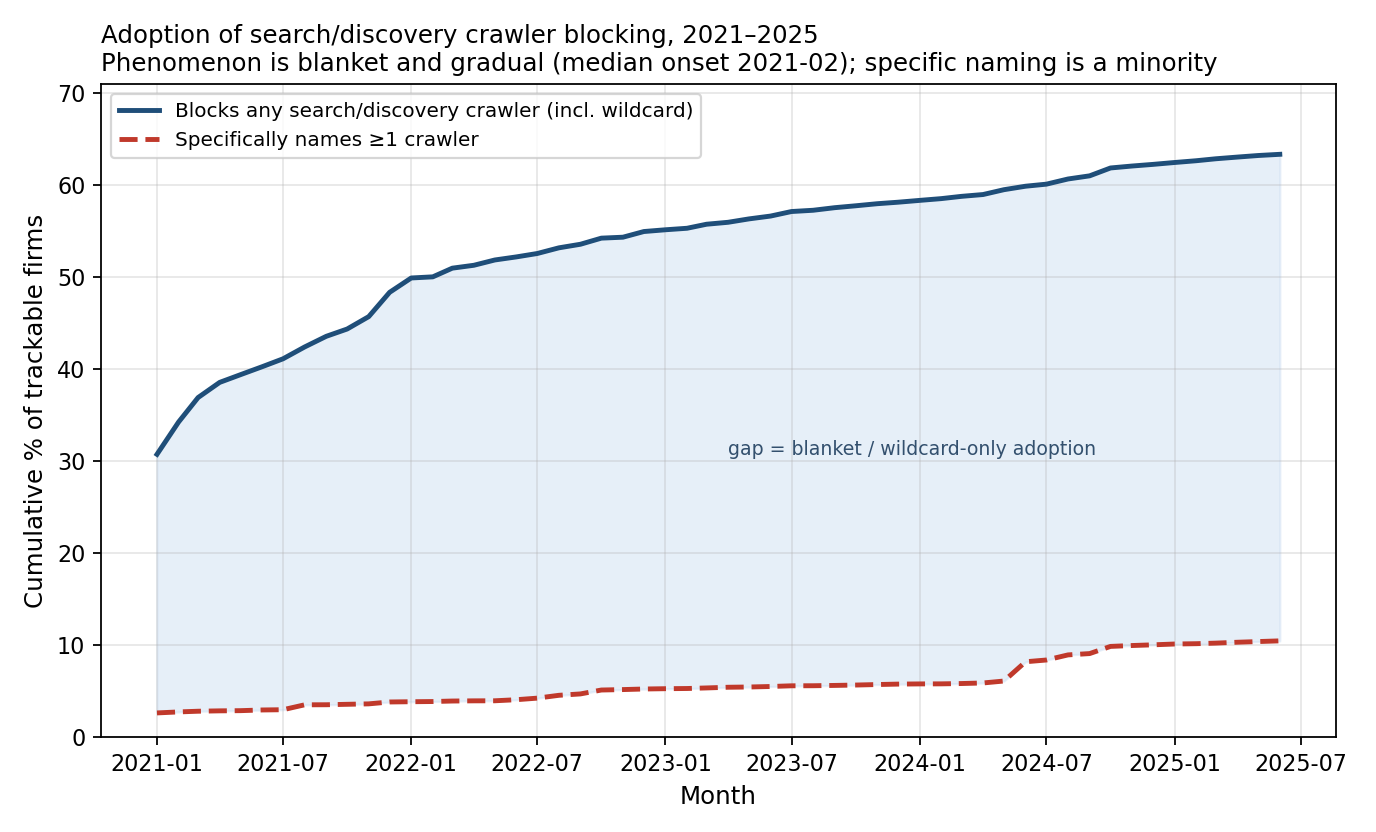
\includegraphics[width=0.92\textwidth]{fig_s2_adoption.png}
\caption{\textbf{Wildcard versus named crawler restrictions, 2021--2025.} Cumulative share of 14{,}615 trackable firms that (i) restrict any of the 31 crawlers (including via a site-wide wildcard) and (ii) name at least one crawler specifically. The wildcard (block-all) share far exceeds explicit per-crawler naming throughout the sample.}
\label{fig:adoption}
\end{figure}

\begin{figure}[t]
\centering
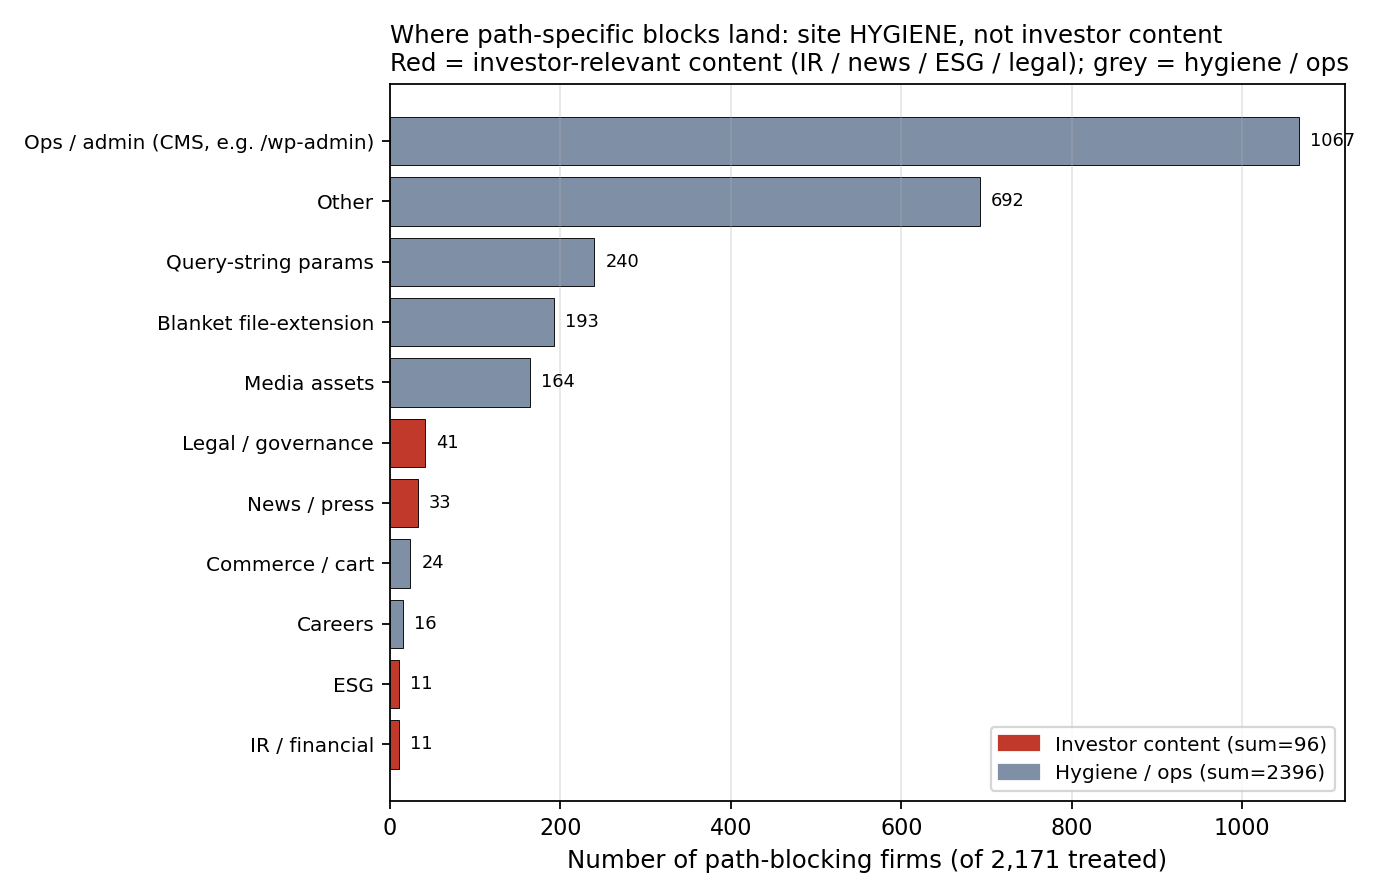
\includegraphics[width=0.92\textwidth]{fig_s2_path_anatomy.png}
\caption{\textbf{Where path-specific restrictions land: site hygiene, not investor content.} Across the 2{,}171 treated firms, path-level restrictions overwhelmingly fall on site-hygiene and operations categories (2{,}396 firm-category blocks) rather than investor-relevant content (96). Categories overlap, so a firm may contribute to several and the counts exceed the number of firms. Paths are sorted into our eleven categories by keyword, following the classification approach of \citet{BoullandBourveauBreuer2026}.}
\label{fig:pathanatomy}
\end{figure}

%==============================================================================
\section{Data and Sample}\label{sec:data}
%==============================================================================

\subsection{Sample and Sources}\label{sec:data_sample}
The unit of observation is a firm filing event: a 10-K or 10-Q filed with the SEC between January 2021 and June 2025. We obtain filing dates from EDGAR, daily returns and dollar volume from CRSP, accounting fundamentals from Compustat, and analyst coverage from I/B/E/S. We reconstruct each firm's monthly crawler-restriction history from archived \texttt{robots.txt} snapshots in the Internet Archive's Wayback Machine and from Common Crawl, as detailed in Section~\ref{sec:data_robots}. Of the 2{,}171 firms in the treatment cohort (Section~\ref{sec:bg}), 722 have a CRSP--Compustat match and at least one valid filing-window observation and so enter the estimation sample, paired with 1{,}186 never-restricting control firms. The resulting sample contains 27{,}327 filing events from 1{,}908 firms.

\subsection{Reconstructing Crawler-Restriction Histories}\label{sec:data_robots}
A firm's \texttt{robots.txt} changes over time and is archived nowhere in its regulatory filings, so we reconstruct each firm's monthly restriction history from the Internet Archive's Wayback Machine, the same historical-web source \citet{BoullandBourveauBreuer2026} use to build their website panels. For each firm we resolve its corporate web domain and query the Wayback Machine's capture index for every archived copy of that domain's \texttt{robots.txt}. The archive crawls sites at irregular intervals, so captures are unevenly spaced; for each calendar month with at least one capture we keep the last capture in the month, which reflects the rule in force at month-end. We parse each captured file into its \texttt{User-agent} groups and \texttt{Disallow} directives and record, for each of the 31 crawlers in each month, whether the firm disallows that crawler at the site root or a sub-path, either by naming the crawler or through an applicable site-wide wildcard group. Months with no Wayback capture are filled from Common Crawl, whose periodic web-scale snapshots we query by host to recover \texttt{robots.txt} files the Wayback Machine missed. A firm's first-restriction month, $m^{\ast}_i$, is the first month in which it disallows any of the 31 crawlers; this onset defines treatment in the next subsection.

\subsection{Independent Variable: Crawler-Access Restriction}\label{sec:data_iv}
Let $\mathit{Block}_i$ equal one if firm $i$ ever restricts any of the 31 crawlers of Table~\ref{tab:crawlers} during the sample, and let $m^{\ast}_i$ denote firm $i$'s first-restriction month. The staggered treatment indicator for filing event $f$ of firm $i$ is
\begin{equation}
\bigl(\mathit{Block}\times\mathit{Post}\bigr)_{i,f}
= \mathbf{1}\!\left[\,\mathit{Block}_i=1 \;\text{and}\; m(f) > m^{\ast}_i\,\right],
\end{equation}
where $m(f)$ is the filing's calendar month. We exclude the firm's filing in its first-restriction month itself (to avoid contaminating the onset), and we restrict the treated group to firms with a clean pre-restriction history (first restriction on or before 2025-06, the sample end). Control firms (``never-restricting'') never restrict any of the 31 crawlers.

\subsection{Dependent Variable: Abnormal Filing-Window Illiquidity}\label{sec:data_dv}
Our liquidity measure is the daily illiquidity ratio of \citet{Amihud2002}, which we denote $\mathit{AIM}$. For firm $i$ on trading day $d$, it is the absolute return per dollar of trading volume,
\begin{equation}
\mathit{AIM}_{i,d} \;=\; \frac{\lvert r_{i,d}\rvert}{\mathit{DolVol}_{i,d}}\times 10^{6},
\end{equation}
where $r_{i,d}$ is the daily return and $\mathit{DolVol}_{i,d}$ is daily dollar volume (price $\times$ share volume); days with non-positive dollar volume are set to missing. Higher $\mathit{AIM}$ means a given dollar of trading moves the price more, i.e.\ lower liquidity.

We measure liquidity in the disclosure window relative to a local pre-filing benchmark, following the abnormal-announcement-window methodology of \citet{Beaver1968}, \citet{LandsmanMaydew2002}, and \citet{LandsmanMaydewThornock2012}. With day $0$ defined as the first trading day on or after the filing date, the event window is $[-1,+1]$ trading days (the announcement-window convention of \citet{LandsmanMaydewThornock2012}), and the benchmark is the local pre-filing window $[-60,-10]$ trading days. Our primary outcome is the within-event abnormal log Amihud,
\begin{equation}
\mathit{AbnAIM}_{i,f}
= \ln\!\Bigl(1+\overline{\mathit{AIM}}^{\,[-1,+1]}_{i,f}\Bigr)
- \ln\!\Bigl(1+\overline{\mathit{AIM}}^{\,[-60,-10]}_{i,f}\Bigr).
\end{equation}
Differencing against the firm's own local window removes the firm's contemporaneous liquidity level, so the outcome isolates the abnormal disclosure-window component. Both windows follow \citet{LandsmanMaydewThornock2012}, whose abnormal-volume and abnormal-volatility measures use an event window of days $[-1,+1]$ and a benchmark of days $[-60,-10]$ and $[+10,+60]$; we take only the pre-event side $[-60,-10]$ of their benchmark, which keeps it close to the event while avoiding overlap with the disclosure window, the post-filing drift, and the adjacent-quarter filing. So that each window mean is computed on enough trading days to be informative, we require at least two valid days in the event window and thirty in the benchmark window, and we winsorize the outcome at the 1st and 99th percentiles within the estimation sample.

\subsection{Controls}\label{sec:data_ctrl}
Our specification includes a compact set of firm-level controls, each a standard determinant of liquidity and each predetermined relative to the filing whose liquidity it conditions. Log total assets and asset tangibility capture firm size and asset structure, which predict the depth of a stock's market and the cost of trading it. Leverage and return on assets capture financial condition and profitability, which move a firm's default and information risk and hence its spread. The market-to-book ratio captures growth and valuation, which shape the mix of informed and uninformed trading. These five accounting characteristics enter at the value from the most recent prior-fiscal-year report available as of the filing month, roughly four months after the firm's fiscal year-end, so the control that conditions a restriction's effect cannot itself have been moved by that restriction. We report a sixth covariate, analyst coverage, $\ln(1+\text{number of estimates})$, measured over the pre-filing window. Analyst attention is itself part of the information environment a restriction may shape, so we do not treat it as an exogenous control: our headline estimate is reported without covariates, and we study coverage directly as an outcome in Section~\ref{app:analyst}. The firm and filing-month fixed effects absorb the permanent level of each characteristic and any variation common to a calendar month, so the controls add only within-firm, off-trend movement, and the estimate is essentially unchanged whether or not they are included (Section~\ref{sec:results}). Each control is winsorized at the 1st and 99th percentiles and mean-centered within the estimation sample.

\subsection{Descriptive Statistics}\label{sec:data_desc}
Table~\ref{tab:summ} reports means by treatment group together with the treated-minus-control difference. Treated and control firms do differ on several observable characteristics: treated firms are smaller (log assets 7.07 vs.\ 7.32), less tangible, more growth-oriented (higher market-to-book), and slightly less profitable, though they are statistically indistinguishable in leverage and analyst coverage. These are level differences, and our design is built precisely to absorb them. Identification comes from the change at a firm's own restriction onset, not from comparing treated firms to control firms: the firm fixed effects difference out every time-invariant gap between the two groups, and the filing-month fixed effects remove variation common to all firms in a month. The cross-sectional imbalance is therefore something we condition away, not a confound we leave open. Consistent with this, the unconditional difference in the abnormal log Amihud is itself small and insignificant ($+0.008$); both groups average a slightly negative abnormal Amihud, reflecting a generally improving liquidity trend over the sample. The effect appears only in the within-firm, post-restriction comparison delivered by the staggered design (Section~\ref{sec:strategy}).

\begin{table}[t]
\centering
\begin{threeparttable}
\caption{Summary statistics, by treatment group}
\label{tab:summ}
\small
\begin{tabular}{lccccc}
\toprule
 & \multicolumn{2}{c}{Treated (restricting)} & \multicolumn{2}{c}{Control (never)} & \\
\cmidrule(lr){2-3}\cmidrule(lr){4-5}
Variable & Mean & SD & Mean & SD & Difference \\
\midrule
Abnormal Amihud (log)              & $-0.018$ & 0.241 & $-0.026$ & 0.287 & $+0.008$ \\
Log assets                          & 7.07     & 2.38  & 7.32     & 2.27  & $-0.26^{**}$ \\
Leverage                            & 0.285    & 0.394 & 0.268    & 0.323 & $+0.017$ \\
Return on assets                    & $-0.144$ & 0.592 & $-0.107$ & 0.576 & $-0.037^{*}$ \\
Market-to-book                      & 5.03     & 9.64  & 4.20     & 8.97  & $+0.83^{**}$ \\
Tangibility                         & 0.380    & 0.399 & 0.449    & 0.450 & $-0.069^{***}$ \\
Analyst coverage (\# estimates)     & 6.94     & 7.74  & 6.43     & 7.16  & $+0.51$ \\
\midrule
Firms                               & \multicolumn{2}{c}{735} & \multicolumn{2}{c}{1{,}212} & \\
Filing events                       & \multicolumn{2}{c}{10{,}464} & \multicolumn{2}{c}{18{,}126} & \\
\bottomrule
\end{tabular}
\begin{tablenotes}\footnotesize
\item \textit{Notes.} Treated firms restrict at least one of the 31 crawlers (Table~\ref{tab:crawlers}) during 2021--2025; control firms never do. Means and standard deviations are over filing events in the analysis sample. The \emph{Difference} column reports the treated-minus-control difference in means; significance is from a regression of each variable on a treated indicator with standard errors clustered by firm, with $^{*}$, $^{**}$, and $^{***}$ denoting $p<0.10$, $0.05$, and $0.01$. The abnormal-Amihud dependent variable is the within-event $[-1,+1]$ minus $[-60,-10]$ log difference, shown unwinsorized. Treated and control firms differ on several observables (size, market-to-book, profitability, and tangibility), so we do not read the raw difference in the dependent variable---itself insignificant---as the treatment effect: identification comes from the staggered design with firm and month fixed effects and time-varying controls (Section~\ref{sec:strategy}), and the headline estimate is reported in Table~\ref{tab:main}. The estimation sample requires a valid filing-window observation and comprises 722 treated and 1{,}186 control firms (27{,}327 filing events).
\end{tablenotes}
\end{threeparttable}
\end{table}


%==============================================================================
\section{Empirical Strategy}\label{sec:strategy}
%==============================================================================
Our baseline specification is a staggered difference-in-differences regression estimated by two-way fixed effects:
\begin{equation}
\mathit{AbnAIM}_{i,f}
= \beta\,\bigl(\mathit{Block}\times\mathit{Post}\bigr)_{i,f}
+ \gamma'\mathbf{X}_{i,f}
+ \alpha_i + \delta_{m(f)} + \varepsilon_{i,f},
\label{eq:twfe}
\end{equation}
where $\alpha_i$ are firm fixed effects, $\delta_{m(f)}$ are filing-month fixed effects, $\mathbf{X}$ collects the controls, and standard errors are clustered by firm. The firm fixed effects absorb every time-invariant difference across firms, including size, industry, listing vintage, business model, and the permanent component of a firm's liquidity, so that $\beta$ is identified entirely from within-firm variation. The filing-month fixed effects absorb shocks common to all firms in a calendar month, including market-wide swings in liquidity, volatility, and trading volume, as well as the secular growth in machine-mediated trading over the 2021--2025 sample, so the estimate is not confounded by aggregate conditions. What remains to identify $\beta$ is the change in a firm's own abnormal filing-window illiquidity after it restricts crawlers, measured against never-restricting firms that file in the same months. Clustering by firm allows the residuals of a firm's repeated filings to be arbitrarily correlated over time.

The two-way fixed-effects estimator is the natural starting point, but a recent econometric literature has shown that it is unreliable in exactly our setting: staggered treatment timing combined with treatment effects that vary across firms or over time. The estimator identifies $\beta$ in part from ``forbidden comparisons'' that use already-restricting firms as controls for newly restricting firms, and it weights the underlying firm-by-period effects with weights that need not be positive. When effects are heterogeneous, these negative weights can attenuate the estimate, and in extreme cases deliver an estimate of the opposite sign to the true average effect \citep{GoodmanBacon2021,deChaisemartinDHaultfoeuille2020}. To address this concern, we re-estimate the effect with the imputation estimator of \citet{BorusyakJaravelSpiess2024}, which fits the firm and time fixed effects on untreated observations only, imputes each treated observation's untreated counterfactual, and averages the resulting gaps. The estimator is robust to treatment-effect heterogeneity, is efficient under standard assumptions, and supplies a 12-period pre-trend test that we report for every outcome. We treat the \citet{BorusyakJaravelSpiess2024} estimate as our preferred specification and the two-way fixed-effects estimate as a transparent benchmark; the estimator of \citet{deChaisemartinDHaultfoeuille2024} serves as a further check. One feature of our design eases these concerns at the outset: because the outcome is already an abnormal, within-event difference, it is pre-trend-clean even where the underlying illiquidity levels are not (Section~\ref{sec:results}).

%==============================================================================
\section{Results}\label{sec:results}
%==============================================================================
Table~\ref{tab:main} reports our central estimate, from the \citet{BorusyakJaravelSpiess2024} imputation estimator (our preferred specification): restricting search and discovery crawlers raises abnormal filing-window illiquidity by $+0.0134$ ($p=0.010$) without controls and $+0.0140$ with the full control set, with a 12-period pre-trend test that does not reject parallel trends ($p=0.48$; Figure~\ref{fig:pretrend}). Because $\mathit{Block}\times\mathit{Post}$ is an indicator, the coefficient is the average effect of a firm's having restricted crawlers, evaluated in its post-restriction filing windows relative to never-restricting controls and to its own pre-restriction filings; it is not a per-unit slope. The control set barely moves the estimate, as the within-event differencing already removes slow-moving firm characteristics. The transparent two-way fixed-effects benchmark is very close ($+0.0109$ without controls, $+0.0111$ with, both $p<0.05$; Table~\ref{tab:twfe_robustness} in the robustness section), so the result does not hinge on the estimator. Under the identifying assumption, we interpret the abnormal-window effect as causal. We report the log specification throughout; the level form and a window-by-window decomposition appear in the robustness section (Table~\ref{tab:eventspec}).

How large is the effect? Because the dependent variable is a within-event difference, the coefficient measures how much a firm's filing-window illiquidity rises relative to its own local benchmark after restriction, not the absolute level of disclosure-window illiquidity. The log coefficient of $0.011$ to $0.013$ corresponds to roughly a one to one-and-a-half percent rise in the one-plus-Amihud ratio at the filing window relative to the firm's own benchmark. In economic terms, the level-form estimate reported in the robustness section (Table~\ref{tab:eventspec}) implies a widening on the order of ten percent of treated firms' benchmark-window Amihud, which averages about $0.30$ (Table~\ref{tab:summ}). By the standards of the microstructure literature these magnitudes are modest. They are, however, precisely estimated, stable across estimators, and (as the next section shows) carry a specific and interpretable market signature rather than a uniform deterioration in liquidity.

This is an abnormal, benchmark-relative effect, and the distinction matters for interpretation. As the robustness section shows (Table~\ref{tab:eventspec}), the filing-window illiquidity level does not rise; rather, treated firms' local benchmark Amihud declines after restriction while the disclosure window fails to improve commensurately, so disclosure windows become relatively more liquidity-constrained than the local benchmark. Throughout, we describe the result as an increase in abnormal, benchmark-relative illiquidity, not as filing windows becoming illiquid in absolute terms.

\begin{table}[t]
\centering
\begin{threeparttable}
\caption{Crawler-access restriction and abnormal filing-window illiquidity}
\label{tab:main}
\small
\begin{tabular}{lcc}
\toprule
 & \multicolumn{2}{c}{Borusyak et al.\ (2024)} \\
\cmidrule(lr){2-3}
 & (1) & (2) \\
\midrule
Crawler block $\times$ Post & $0.0134^{***}$ & $0.0140^{***}$ \\
                            & (0.0052)       & (0.0051) \\
Pre-trend $p$ (12 period)   & 0.48           & 0.52 \\
\midrule
Controls         & No   & Yes \\
Firm FE          & Yes  & Yes \\
Filing-month FE  & Yes  & Yes \\
Observations     & 25{,}516 & 25{,}516 \\
\bottomrule
\end{tabular}
\begin{tablenotes}\footnotesize
\item \textit{Notes.} The dependent variable is the abnormal filing-window Amihud illiquidity (Eq.~\ref{eq:twfe}): the log difference between the $[-1,+1]$ trading-day event window and the $[-60,-10]$ local benchmark. We report the \citet{BorusyakJaravelSpiess2024} imputation estimator as our primary specification, without (column~1) and with (column~2) the control set, each with a 12-period pre-trend test; 580 treated firms and 25{,}516 firm-filings. The control set (log assets, leverage, ROA, market-to-book, tangibility, and analyst coverage, winsorized and within-sample demeaned) barely moves the estimate, because the dependent variable is already an abnormal, within-event difference that nets out slow-moving firm characteristics. The transparent two-way fixed-effects benchmark is very close ($+0.0109$ to $+0.0111$, $p<0.05$) and is reported in the robustness section (Table~\ref{tab:twfe_robustness}); the level form and a window-by-window decomposition are also there (Table~\ref{tab:eventspec}). Standard errors clustered by firm in parentheses. $^{*}$, $^{**}$, $^{***}$ denote significance at the 10\%, 5\%, and 1\% levels.
\end{tablenotes}
\end{threeparttable}
\end{table}


\begin{figure}[t]
\centering
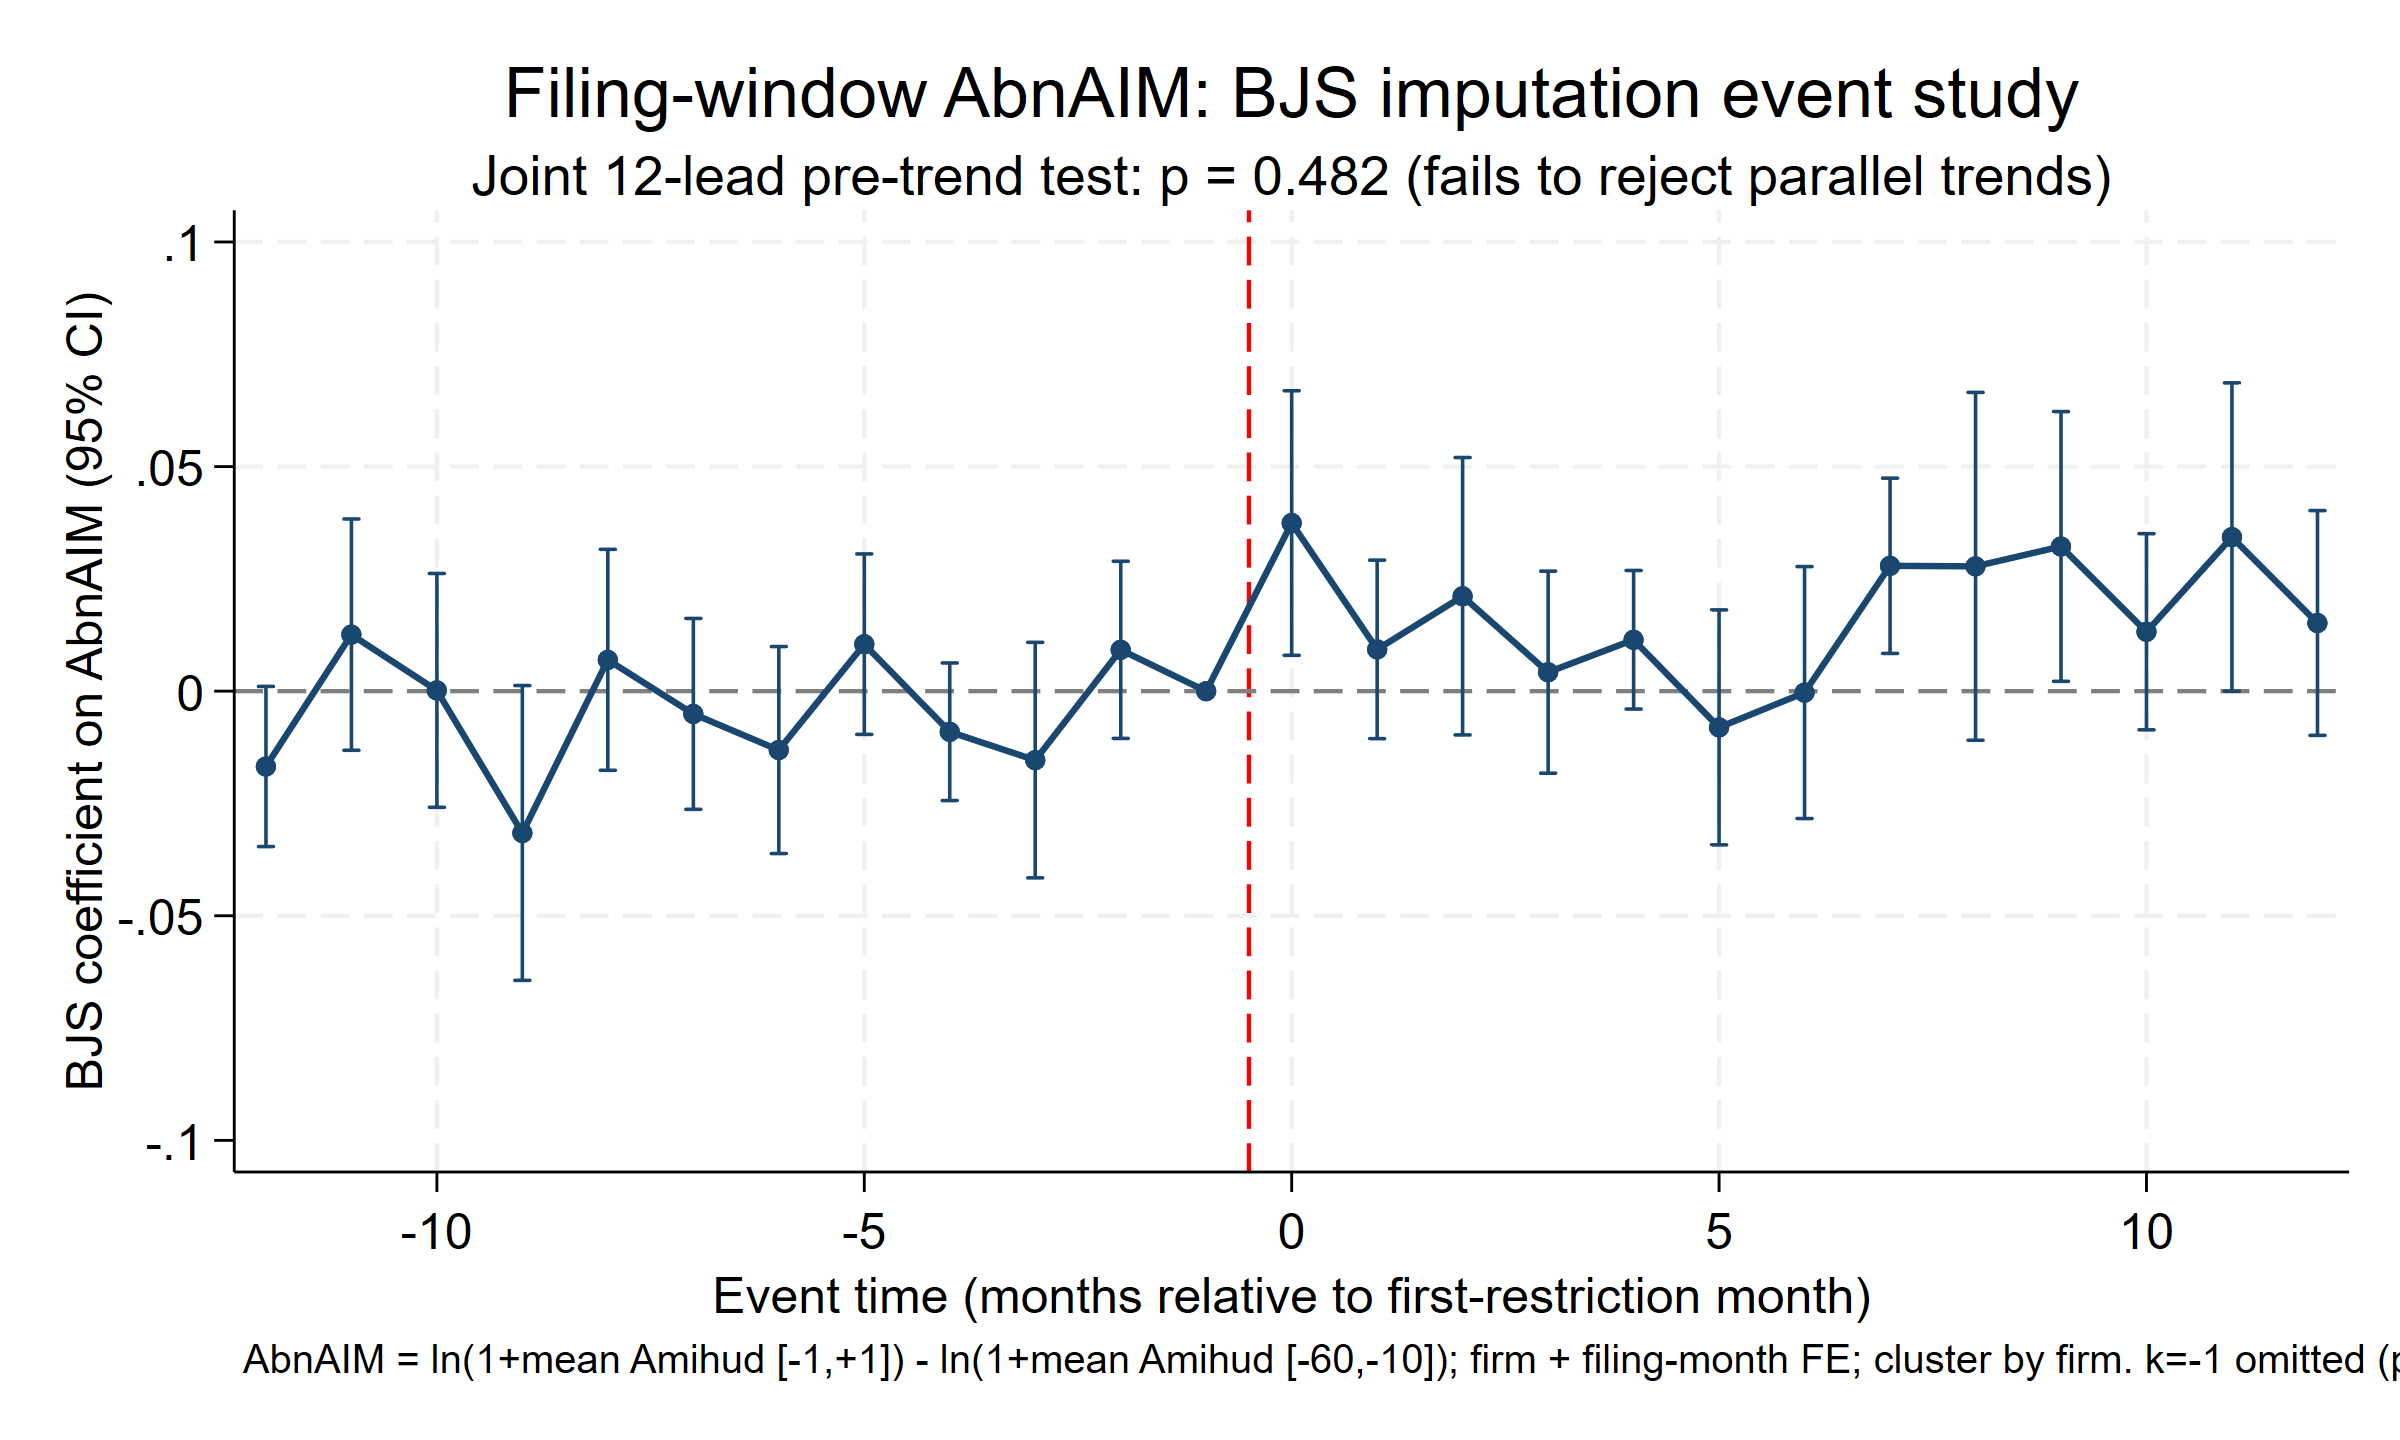
\includegraphics[width=0.9\textwidth]{fig_amihud_bjs_pretrend.png}
\caption{\textbf{Parallel-trends event study for the headline effect.} \citet{BorusyakJaravelSpiess2024} imputation event-study coefficients on abnormal filing-window illiquidity ($\mathit{AbnAIM}$), plotted against event time in months relative to a firm's first-restriction month. The event-window days $[-1,+1]$ and the benchmark days $[-60,-10]$ are integrated inside $\mathit{AbnAIM}$, so the time axis here is the filing's calendar month relative to onset, not a trading day. The omitted reference period is the month before restriction ($k=-1$, pinned at zero), and the red line marks the onset. Whiskers are 95\% confidence intervals from firm-clustered standard errors. The twelve pre-restriction coefficients are jointly insignificant (joint pre-trend test $p=0.48$), consistent with parallel trends; the abnormal effect appears at and after the restriction month.}
\label{fig:pretrend}
\end{figure}

%==============================================================================
\section{Why Does Abnormal Filing-Window Illiquidity Increase?}\label{sec:mech}
%==============================================================================
This section asks what the deterioration is and what it is not.

\subsection{A Price-Impact Channel, Not Spreads or Participation}\label{sec:mech_sig}
The headline says abnormal filing-window illiquidity rises. This subsection asks what kind of illiquidity it is, because the word can mean very different things and our measure does not separate them on its own.

Start with the measure. The Amihud ratio \citep{Amihud2002} is the absolute return divided by dollar volume, $|r|/\mathit{DolVol}$, how far the price moves per dollar traded. It is a daily, low-frequency proxy for price impact in the sense of \citet{Kyle1985}, the slope that links order flow to price; the standard validations confirm that this daily proxy tracks the price-impact benchmarks built from intraday data, with \citet{GoyenkoHoldenTrzcinka2009} finding that ``the Amihud measure does well measuring price impact'' and \citet{Hasbrouck2009} showing that effective costs estimated from daily prices line up closely with their transaction-level counterparts. A higher ratio can come from either side of this fraction. The denominator can fall, as investors withdraw and trade thins. Or the numerator, the absolute return, can grow, and it can grow for two distinct reasons: a wider bid--ask spread inflates the measured return through bid--ask bounce \citep{Roll1984}, even with no change in price impact, or the same disclosure genuinely moves the price more. We take each in turn.

It is not the spread. Posted quoted spreads and two low-frequency spread proxies do not move after restriction (Table~\ref{tab:excl}), so whatever raises the ratio, it is not a wider cost of crossing the bid--ask. It is not a withdrawal of trade. The dollar-volume denominator rises rather than falls ($+0.061$, $p=0.020$ under the imputation estimator, and positive though not significant under two-way fixed effects); trading activity in the disclosure window goes up, so the illiquidity is not investors stepping away. What rises is the size of the price move itself. Return variance is the classic gauge of how strongly a disclosure moves prices \citep{Beaver1968}; its abnormal, filing-window form (the average squared market-adjusted daily return, relative to the firm's own benchmark) increases ($+0.121$, $p=0.015$; Table~\ref{tab:signature}), and it is the one part of the signature significant under both the imputation estimator and the two-way fixed-effects benchmark: relative to the firm's own pre-filing benchmark, the disclosure window carries a larger price response, while trading neither thins nor faces wider spreads.

The pieces point one way. Relative to the firm's own pre-filing benchmark, a dollar of trading in the disclosure window moves the price more, while spreads do not widen and volume does not contract. This is a price-impact, or equivalently a market-depth, effect in the sense of \citet{Kyle1985}, where lower depth is a steeper price-impact slope. This is what one would expect if restricting machine-mediated discovery raises the cost of incorporating the filing, so that trading on it is more adverse-selecting and moves prices further, in the logic of \citet{GlostenMilgrom1985}. Two cautions sharpen the reading. Prices do not incorporate the filing more slowly: there is no post-filing drift (Table~\ref{tab:excl}), so this is a larger price impact at the event, not delayed or incomplete incorporation. And the joint rise in variance and volume is also consistent with investors interpreting the filing more heterogeneously, a disagreement reading we test directly but can only call suggestive (Appendix~\ref{app:disagree}).

\begin{table}[t]
\centering
\begin{threeparttable}
\caption{The price-impact signature: return variance and trading volume}
\label{tab:signature}
\small
\begin{tabular}{lcc}
\toprule
 & \multicolumn{2}{c}{Borusyak et al.\ (2024)} \\
\cmidrule(lr){2-3}
 & (1) & (2) \\
\midrule
\textit{Abnormal return variance} & & \\
\quad Crawler block $\times$ Post & $0.121^{**}$ & $0.111^{**}$ \\
                                  & (0.050)      & (0.050) \\
\quad Pre-trend $p$ (12 period)   & 0.52         & 0.53 \\[4pt]
\textit{Abnormal dollar volume}   & & \\
\quad Crawler block $\times$ Post & $0.061^{**}$ & $0.054^{**}$ \\
                                  & (0.026)      & (0.026) \\
\quad Pre-trend $p$ (12 period)   & 0.83         & 0.83 \\
\midrule
Controls         & No       & Yes \\
Firm FE          & Yes      & Yes \\
Filing-month FE  & Yes      & Yes \\
Observations     & 25{,}516 & 25{,}516 \\
\bottomrule
\end{tabular}
\begin{tablenotes}\footnotesize
\item \textit{Notes.} Each panel reports the \citet{BorusyakJaravelSpiess2024} imputation estimate of the effect of crawler restriction on an abnormal filing-window outcome, without (column~1) and with (column~2) the control set, each with a 12-period pre-trend test. Each outcome is an abnormal within-event difference in the same form as the headline (Table~\ref{tab:main}): the log of the event-window average over days $[-1,+1]$ minus the log of the local-benchmark average over days $[-60,-10]$. Return variance uses the mean squared market-adjusted daily return; dollar volume uses mean daily dollar volume. The two-way fixed-effects benchmark is similar (return variance $+0.099$, $p=0.02$; dollar volume $+0.026$, $p=0.20$, the latter positive but not significant). The third leg of the signature, posted and proxy spreads, is null and reported in Table~\ref{tab:excl}. The control set, fixed effects, and estimation sample match Table~\ref{tab:main}. Standard errors clustered by firm in parentheses. $^{*}$, $^{**}$, $^{***}$ denote significance at the 10\%, 5\%, and 1\% levels.
\end{tablenotes}
\end{threeparttable}
\end{table}


\subsection{Where the Effect Is Strongest: Younger Firms}\label{sec:mech_locus}
To locate the effect we interact the treatment with predetermined, $z$-scored firm characteristics in a moderated difference-in-differences,
\begin{equation}
\mathit{AbnAIM}_{i,f} = \beta_1\,(\mathit{Block}\times\mathit{Post})_{i,f} + \beta_2\,(\mathit{Block}\times\mathit{Post}\times Z_i) + \alpha_i + \delta_{m(f)} + \varepsilon_{i,f},
\label{eq:locus}
\end{equation}
where $Z_i$ is the moderator (firm age, analyst coverage, size, or EDGAR attention), measured over the pre-restriction window. The firm fixed effects $\alpha_i$ absorb the level of $Z_i$ and the $\mathit{Block}\times Z_i$ interaction (both fixed within firm); because control firms are never treated, there is no separate $\mathit{Post}\times Z$ term, and $\beta_2$ measures how the post-restriction jump scales with the moderator. The interaction is identified only under two-way fixed effects, so this is a descriptive locating exercise rather than a heterogeneity-robust causal claim.

Table~\ref{tab:locus} reports each moderator in its own column. The effect concentrates among younger firms: the age interaction is negative and significant ($-0.0151$, $p=0.06$ alone in column~1; $-0.0184$, $p=0.04$ jointly in column~5). The base and age-interaction coefficients nearly cancel, so a firm one standard deviation older than the mean shows essentially no effect; the effect lives in the younger firms. Analyst coverage, size, and EDGAR attention are each individually insignificant (columns~2--4), and the age interaction survives entering them jointly (column~5); separate horse races against institutional ownership, retail float, and filing-package size (not tabulated) leave it unchanged. We read age as a condition, an immature information environment, rather than a separate causal channel; the young-treated cell is thin and the interaction carries no parallel-trends test, so we do not over-read the magnitude.

\begin{table}[t]
\centering
\begin{threeparttable}
\caption{Where the effect is strongest: firm age and other moderators}
\label{tab:locus}
\footnotesize
\setlength{\tabcolsep}{4pt}
\begin{tabular}{lccccc}
\toprule
 & (1) & (2) & (3) & (4) & (5) \\
Moderator $Z$: & Age & Coverage & Size & EDGAR & Joint \\
\midrule
Crawler block $\times$ Post        & $0.0156^{**}$ & $0.0108$ & $0.0101^{*}$ & $0.0097$ & $0.0185^{**}$ \\
                                   & (0.0065)      & (0.0070) & (0.0057)     & (0.0061) & (0.0077) \\
\quad $\times$ Log(firm age)       & $-0.0151^{*}$ &          &              &          & $-0.0184^{**}$ \\
                                   & (0.0079)      &          &              &          & (0.0087) \\
\quad $\times$ Analyst coverage    &               & $-0.0025$ &             &          & $-0.0145$ \\
                                   &               & (0.0069)  &             &          & (0.0094) \\
\quad $\times$ Log(size)           &               &           & $0.0028$    &          & $0.0179^{*}$ \\
                                   &               &           & (0.0070)    &          & (0.0108) \\
\quad $\times$ EDGAR attention     &               &           &             & $0.0020$ & \\
                                   &               &           &             & (0.0066) & \\
\midrule
Firm FE          & Yes & Yes & Yes & Yes & Yes \\
Filing-month FE  & Yes & Yes & Yes & Yes & Yes \\
Treated firms    & 722 & 604 & 628 & 604 & 583 \\
Firm clusters    & 1{,}908 & 1{,}790 & 1{,}814 & 1{,}790 & 1{,}769 \\
Observations     & 27{,}327 & 26{,}104 & 26{,}627 & 26{,}104 & 25{,}977 \\
\bottomrule
\end{tabular}
\begin{tablenotes}\footnotesize
\item \textit{Notes.} Each column estimates the moderated difference-in-differences of Eq.~\eqref{eq:locus}: the dependent variable is the abnormal filing-window Amihud (log), and the reported $\times Z$ row is the triple interaction $\mathit{Block}\times\mathit{Post}\times Z$, where $Z$ is a predetermined, $z$-scored firm characteristic measured before restriction (so the coefficient is the change in the treatment effect per one-standard-deviation increase in $Z$). Firm fixed effects absorb the level of $Z$ and $\mathit{Block}\times Z$; there is no separate $\mathit{Post}\times Z$ term because controls are never-treated. Columns (1)--(4) enter one moderator at a time, each on the firms that carry that moderator (hence the differing treated counts); column (5) enters age, coverage, and size jointly. The negative, significant age interaction---robust to the joint specification---means the effect is stronger among younger firms; coverage, size, and EDGAR attention are individually insignificant. These interactions are estimated by two-way fixed effects (the imputation estimator does not estimate interactions) and carry no parallel-trends test; the young-treated cell is thin, so the joint column is read with caution. Standard errors clustered by firm in parentheses. $^{*}$, $^{**}$, $^{***}$ denote 10\%, 5\%, 1\%.
\end{tablenotes}
\end{threeparttable}
\end{table}


\subsection{Interpretation}\label{sec:mech_interp}
Taken together, the deterioration is best read as a price-impact / market-depth effect in the spirit of \citet{Kyle1985}: the same disclosure moves prices more per dollar traded, concentrated where information environments are immature (the younger firms of Section~\ref{sec:mech_locus}), with the adjacent alternatives (delayed diffusion, analyst delay, spread widening, volume withdrawal, EDGAR substitution, and AI-crawler specificity) each excluded (Section~\ref{sec:rob}).
%==============================================================================
\section{Robustness}\label{sec:rob}
%==============================================================================
\subsection{The headline is a benchmark-relative, pre-trend-clean effect}\label{app:eventspec}
Because the outcome is a within-event difference between the filing window and a local benchmark, it is worth asking which leg moves. Table~\ref{tab:eventspec} regresses the two levels separately on the treatment. The filing-window absolute level does not rise (it is slightly negative and fails its own parallel-trends test, $p\approx0.004$), while the local benchmark level declines with a clean pre-trend. The positive headline is therefore the benchmark level falling faster than the filing window: disclosure windows do not share in the firm's broadly improving local liquidity. Only the abnormal difference (the headline) is pre-trend-clean (log $p=0.48$, level $p=0.38$), which is why we build inference on it and describe the effect throughout as benchmark-relative rather than as an absolute rise in filing-window illiquidity.

\begin{table}[t]
\centering
\begin{threeparttable}
\caption{Event-specificity: the headline effect is benchmark-relative}
\label{tab:eventspec}
\small
\begin{tabular}{lcccc}
\toprule
 & \multicolumn{2}{c}{Abn.\ Amihud (log)} & \multicolumn{2}{c}{Abn.\ Amihud (level)} \\
\cmidrule(lr){2-3}\cmidrule(lr){4-5}
Window & Coef. & Pre-trend $p$ & Coef. & Pre-trend $p$ \\
\midrule
Filing-window level $[-1,+1]$    & $-0.008$        & 0.004 & $-0.018$        & 0.004 \\
Benchmark level $[-60,-10]$      & $-0.025^{**}$   & 0.24  & $-0.066^{***}$  & 0.22  \\
Abnormal (difference; headline)  & $+0.013^{**}$   & 0.48  & $+0.039^{***}$  & 0.38  \\
\bottomrule
\end{tabular}
\begin{tablenotes}\footnotesize
\item \textit{Notes.} Each cell is a \citet{BorusyakJaravelSpiess2024} estimate of Crawler block $\times$ Post on the indicated quantity (firm and filing-month fixed effects; 580 treated firms), with its 12-period pre-trend $p$. The filing-window absolute level does \emph{not} rise and fails its own pre-trend ($p\approx0.004$); the local benchmark level declines with a clean pre-trend; by construction the abnormal difference equals the filing level minus the benchmark level. Only the difference (the headline) is pre-trend-clean, which is why we build on it: the positive headline is a benchmark-relative effect---disclosure windows do not share in the firm's improving local liquidity---not an absolute rise in filing-window illiquidity.
\end{tablenotes}
\end{threeparttable}
\end{table}


\subsection{The effect is not an earnings-announcement artifact}\label{app:earnings}
In the EDGAR era the filing date and the earnings announcement are systematically confounded. \citet{LiRamesh2009} show that the apparent market reaction on the periodic-report filing date is largely an artifact of this disclosure endogeneity: once filings that coincide with the first earnings release are removed, the 10-Q filing-date reaction disappears, and the surviving 10-K reaction concentrates in calendar-quarter-end clusters rather than in the filing's information content. A natural concern is therefore that our filing-window illiquidity effect is an earnings-announcement effect in disguise. Table~\ref{tab:earnings} confronts this directly, and the effect does not behave as the artifact would. It is not concentrated in filings that coincide with the announcement (Panel~A): the concurrent cell, though the best powered, is the weakest. Dropping all earnings-concurrent filings and re-estimating on the non-concurrent subsample (Panel~B) leaves the effect intact (TWFE $+0.0102$, $p=0.029$; \citet{BorusyakJaravelSpiess2024} $+0.0072$, $p=0.043$, with a clean pre-trend), and adding an earnings-window indicator to the matched-sample headline does not absorb it (Panel~C). Finally, re-anchoring the entire design on the announcement date itself, with day~0 at the announcement and identical windows and treatment, yields a null ($+0.0034$, s.e.\ $0.0033$, pre-trend $p=0.71$; Panel~D) despite being well powered: its 80\% minimum detectable effect, $0.0094$, is smaller than the filing-anchored estimate. The abnormal-illiquidity response is anchored to the filing, not to the announcement. The effect is individually significant among the more frequent quarterly (10-Q) filings and not among annual (10-K) filings, but the two are not statistically distinguishable, so we read this as a frequency pattern rather than a form-specific mechanism.

That a crawler restriction moves disclosure-window liquidity net of the announcement is consistent with a literature showing that periodic filings carry incremental, separately processed information. \citet{LiNekrasovTeoh2020} document that material withheld at the announcement and released only in the subsequent filing is under-reacted to, with analysts deferring forecasts until after the filing; \citet{CohenMalloyNguyen2020} find that changes in 10-K text predict future returns even though they produce no announcement-date reaction, evidence that filing content is incorporated slowly and separately from the announcement. The growing tendency to bundle earnings information with the filing itself \citep{ArifMarshallSchroederYohn2019} is exactly what makes the two events necessary to separate, as \citet{LiRamesh2009} urge; our concurrent-versus-non-concurrent design does so, and the effect survives. The filing window is thus a genuine information event in its own right, so a restriction that raises the cost of processing the filing can affect disclosure-window liquidity even after the announcement is accounted for.

\begin{table}[t]
\centering
\begin{threeparttable}
\caption{The effect is not an earnings-announcement artifact}
\label{tab:earnings}
\small
\begin{tabular}{lc}
\toprule
 & Abn.\ Amihud (log) \\
\midrule
\multicolumn{2}{l}{\textit{Panel A: By proximity to the earnings announcement (Borusyak et al.\ 2024)}}\\[2pt]
Concurrent ($|\text{filing}-\text{rdq}|\le 1$)   & $+0.0036$\ (0.44) \\
Mid (2--10 days)                                  & $+0.0069$\ (0.086) \\
Standalone ($>10$ days)                           & $+0.0066$\ (0.32) \\[4pt]
\multicolumn{2}{l}{\textit{Panel B: Drop earnings-concurrent filings (non-concurrent subsample)}}\\[2pt]
\quad TWFE                                        & $0.0102^{**}$\ (0.0046) \\
\quad Borusyak et al.\ (2024)                     & $0.0072^{**}$\ (0.0035) \\
\quad\quad Borusyak et al.\ pre-trend $p$         & 0.56 \\[4pt]
\multicolumn{2}{l}{\textit{Panel C: Earnings-window control on the matched sample (TWFE)}}\\[2pt]
Crawler block $\times$ Post (net of EA dummy)     & $0.0061$\ (0.0038) \\[4pt]
\multicolumn{2}{l}{\textit{Panel D: Re-anchored on the earnings announcement (Borusyak et al.\ 2024)}}\\[2pt]
Announcement-anchored $\mathit{AbnAIM}$           & $0.0034$\ (0.0033) \\
\quad Pre-trend $p$; 80\% MDE                     & 0.71;\ 0.0094 \\
\bottomrule
\end{tabular}
\begin{tablenotes}\footnotesize
\item \textit{Notes.} The filing panel is entirely periodic reports (10-K/10-Q). Filing events are matched to the nearest Compustat earnings-announcement date (rdq) within an own-quarter window; ``concurrent'' filings are filed within one day of the announcement. Panel~A reports the Borusyak et al.\ (2024) estimate (with the coefficient $p$-value in parentheses) by proximity; the effect is not concentrated in concurrent filings. Panel~B re-estimates the headline on the non-concurrent subsample (filings filed more than one day from the announcement, within the matched-rdq sample; 313 treated firms): the effect survives with a clean pre-trend. Panel~C adds an earnings-window indicator to the matched-sample headline; standard errors clustered by firm in parentheses. Panel~D re-anchors the entire design on the earnings-announcement date: day~0 is the first trading day on or after rdq, with identical windows, outcome construction, and treatment timing (76{,}696 announcement events; 567 treated firms in the imputation panel). The estimate is a null with a clean pre-trend, and the test is well powered: its 80\% minimum detectable effect (0.0094) is below the filing-anchored estimate ($+0.0134$). The effect is individually significant among 10-Q filings (Borusyak et al.\ 2024 $+0.0129$, $p=0.026$) and not among 10-K filings ($+0.0056$, $p=0.40$), but the two are not statistically distinguishable (form interaction $p=0.76$), so we do not read a form-specific mechanism. $^{*}$, $^{**}$, $^{***}$ denote 10\%, 5\%, 1\%.
\end{tablenotes}
\end{threeparttable}
\end{table}


\subsection{Channels ruled out}\label{app:excl}
Table~\ref{tab:excl} collects the channels we can exclude. Not delayed price incorporation. A post-filing drift test over $[+2,+10]$ shows no delayed incorporation: the delayed-response share is a precise null (\citet{BorusyakJaravelSpiess2024} $-0.002$, $p=0.73$, pre-trend $p=0.51$), and signed drift is null; the test bounds the $[+2,+10]$ drift, not slowing within $[-1,+1]$ or beyond $+10$. Not posted-spread widening or lower participation. Posted quoted spreads and two low-frequency spread proxies \citep{CorwinSchultz2012,AbdiRanaldo2017} are null, and trading activity rises rather than falls (Section~\ref{sec:mech_sig}); the illiquidity is Amihud / price-impact, not a posted-spread channel. Not disclosure substitution. Abnormal EDGAR access to the treated firms' filings, in the same abnormal form, is null across periodic, 10-K, and 8-K access (\citet{BorusyakJaravelSpiess2024}, $p>0.45$); investors do not compensate by reading the filings directly. Not AI/LLM-specific. Restricting the treatment to the AI-search crawlers among the 31 yields underpowered, insignificant estimates, while a non-AI placebo arm of low-reliance traditional crawlers is itself significant; because most firms restrict every crawler at once through a site-wide wildcard, the data cannot attribute the effect to AI crawlers specifically, and we read the treatment as a restriction on machine-mediated discovery in general (Appendix~\ref{app:aiplacebo}). Not template churn or IR-page targeting. Restrictions are broad across path types rather than concentrated in investor-content paths, and explicit blocks of investor-relations or financial-document paths are rare (Figure~\ref{fig:pathanatomy}).

\begin{table}[t]
\centering
\begin{threeparttable}
\caption{Channels ruled out}
\label{tab:excl}
\footnotesize
\setlength{\tabcolsep}{4pt}
\begin{tabular}{@{}llcc@{}}
\toprule
Channel / outcome & Estimator & Estimate (s.e.) & Pre-trend \\
\midrule
\multicolumn{4}{l}{\textit{Delayed price incorporation}}\\
\quad Delayed $|$return$|$ share $[+2,+10]$ & Borusyak et al.\ & $-0.002$\ (0.005)   & 0.51 \\
\quad Signed post-filing drift              & Borusyak et al.\ & $0.003$\ (0.003)    & 0.24 \\[3pt]
\multicolumn{4}{l}{\textit{Posted spreads}}\\
\quad Abnormal quoted spread                & Borusyak et al.\ & $-0.00002$\ (0.0001)& ---  \\
\quad Corwin--Schultz spread                & Borusyak et al.\ & $0.00004$\ (0.0005) & 0.27 \\
\quad Abdi--Ranaldo spread                  & Borusyak et al.\ & $-0.0005$\ (0.0008) & 0.14 \\[3pt]
\multicolumn{4}{l}{\textit{Trading volume / substitution}}\\
\quad Share volume $[0,+5]$                 & Borusyak et al.\ & $-0.019$\ (0.063)   & ---  \\
\quad EDGAR access, periodic filings        & Borusyak et al.\ & $-0.033$\ (0.030)   & 0.31 \\
\quad EDGAR access, 10-K                    & Borusyak et al.\ & $-0.022$\ (0.030)   & 0.79 \\[3pt]
\multicolumn{4}{l}{\textit{AI-specificity}}\\
\quad AI-crawler restriction (log)          & TWFE & $-0.005$\ (0.018)   & ---  \\
\quad Non-AI placebo (log)                  & TWFE & $0.020^{**}$\ (0.009)& ---  \\
\bottomrule
\end{tabular}
\begin{tablenotes}\footnotesize
\item \textit{Notes.} Each row is a separate regression of the indicated outcome on Crawler block $\times$ Post, with the same firm and filing-month fixed effects (specifications described in the text). The imputation rows report the \citet{BorusyakJaravelSpiess2024} estimator with its 12-period pre-trend $p$; ``---'' indicates the pre-trend is not reported for that source (the spread and volume rows are from a broader cross-firm channel map on a different treatment definition). The AI-crawler rows restrict the treatment to firms naming AI-search crawlers (OpenAI, Anthropic, Perplexity, DuckDuckGo; expanded set adds You.com, Andi, Amazon); these arms are underpowered, while a non-AI placebo arm is itself significant, so the effect cannot be attributed to AI crawlers specifically. Standard errors in parentheses. $^{*}$, $^{**}$, $^{***}$ denote 10\%, 5\%, 1\%.
\end{tablenotes}
\end{threeparttable}
\end{table}


\subsection{Estimator robustness}\label{app:did}
We report the \citet{BorusyakJaravelSpiess2024} imputation estimator as our primary specification throughout, precisely because two-way fixed effects is unreliable under staggered timing \citep{GoodmanBacon2021,deChaisemartinDHaultfoeuille2020} (Section~\ref{sec:strategy}). Table~\ref{tab:twfe_robustness} gives the two-way fixed-effects benchmark for the headline; it coincides with the imputation estimate to within rounding, so the staggered-timing bias is not driving the result. The interaction exhibits (the moderator interactions of Section~\ref{sec:mech_locus}) are necessarily two-way fixed-effects estimates, because the imputation estimator does not estimate interaction terms; we flag this where it applies and treat them as descriptive, without a parallel-trends test on the interaction. For the few-treated-cluster crawler-type arms of Appendix~\ref{app:aiplacebo}, we confirm inference with a wild-cluster bootstrap (Webb weights), under which the significant non-AI placebo arm survives.

\begin{table}[t]
\centering
\begin{threeparttable}
\caption{Two-way fixed-effects benchmark for the headline}
\label{tab:twfe_robustness}
\small
\begin{tabular}{lcc}
\toprule
 & \multicolumn{2}{c}{TWFE} \\
\cmidrule(lr){2-3}
 & (1) & (2) \\
\midrule
Crawler block $\times$ Post & $0.0109^{**}$ & $0.0111^{**}$ \\
                            & (0.0051)      & (0.0051) \\
Within-$R^2$                & 0.000         & 0.002 \\
\midrule
Controls         & No   & Yes \\
Firm FE          & Yes  & Yes \\
Filing-month FE  & Yes  & Yes \\
Observations     & 27{,}327 & 27{,}327 \\
\bottomrule
\end{tabular}
\begin{tablenotes}\footnotesize
\item \textit{Notes.} Two-way fixed-effects estimate of the headline abnormal filing-window Amihud (Eq.~\ref{eq:twfe}; firm and filing-month fixed effects, standard errors clustered by firm), without and with the control set. We report the \citet{BorusyakJaravelSpiess2024} imputation estimator as the primary specification (Table~\ref{tab:main}); the two coincide to within rounding, which is the point of this table. Within-$R^2$ is small by construction (a single difference-in-differences indicator net of firm and month fixed effects). $^{*}$, $^{**}$, $^{***}$ denote 10\%, 5\%, 1\%.
\end{tablenotes}
\end{threeparttable}
\end{table}


%==============================================================================
\section{Conclusion}\label{sec:concl}
%==============================================================================
As the discovery of corporate disclosure migrates from human readers to machine intermediaries, a firm's control over those machines becomes part of its information environment. We document one consequence. When a firm restricts the search and discovery crawlers that index its website, the price impact of its mandatory filings rises in the days around each filing, concentrated among younger firms and showing up in price-impact and return-variance measures rather than in posted spreads, a withdrawal of trading, delayed price incorporation, or substitution toward EDGAR. The restriction never touches the filing on EDGAR; what it raises is the cost of finding and contextualizing the same disclosure through the channels investors increasingly use.

We read this as consistent with a discoverability-driven price-impact effect rather than as a fully identified channel, and the honest limit of the evidence marks the natural next step. A first stage measured on the treated crawlers themselves (a firm's presence and ranking in the search and answer surfaces those crawlers feed, or fetch-level access logs around the restriction date) would turn a consistent-with reading into a tested mechanism. As firms increasingly decide whether to let machines, including AI systems, crawl their disclosures, the terms of that access may turn out to be a quietly consequential disclosure choice.

%==============================================================================
\appendix
%==============================================================================
\section{Supplementary Robustness and Diagnostics}\label{sec:appendix}

\subsection{Naming specificity: does naming a crawler change the effect?}\label{app:anatomy}
A natural question is whether the effect is a property of crawler restriction in general or of some narrow, deliberately targeted restriction. The latter would undercut the exogeneity argument of Section~\ref{sec:bg_why}, which rests on the typical restriction being a blanket, content-agnostic act. Table~\ref{tab:anatomy} examines a predetermined feature of the restriction measured at its onset: whether the firm names a specific crawler or relies only on a \texttt{User-agent: *} wildcard.

Naming specificity does not change the effect. The within-treated differential on naming a crawler is a precise zero ($-0.0065$, $p=0.53$ in logs), so we cannot distinguish firms that name a crawler from those that restrict only through a wildcard. Estimated as separate cohorts against the same never-restricting controls, the wildcard-only arm, which is 88\% of the treated firms and exactly the content-agnostic population that motivates our identifying assumption, reproduces the headline with a clean pre-trend. The names-specific arm is statistically null but positive and same-signed, with pre-trends that do not reject. We read its nulls as a power limitation rather than evidence of absence: the arm contains 82 firms, and 56 once we further require the absence of any wildcard, so its minimum detectable effect at 80\% power is several times the headline. Two cautions keep us from over-reading the wildcard arm. Because it is the large majority of the sample, its agreement with the headline is in part mechanical. More substantively, a specific \texttt{Disallow} layered on an existing wildcard removes nothing the wildcard had not already removed, so we would not expect naming, on its own, to carry an independent effect. The appropriate reading is that the effect operates through the blanket restriction and is invariant to whether a crawler is named, consistent with the content-agnostic motive of Section~\ref{sec:bg_why}; it is not a finding that wildcards are causal while names are inert.

\begin{table}[t]
\centering
\begin{threeparttable}
\caption{Naming specificity: wildcard-only vs.\ named crawlers}
\label{tab:anatomy}
\small
\begin{tabular}{lc}
\toprule
 & Abn.\ Amihud (log) \\
\midrule
\textit{Within-treated differential (TWFE):} & \\
\quad Names-specific $\times$ Post                 & $-0.0065$\ (0.0104) \\[2pt]
\textit{Split sample, arm vs.\ never-restricting controls:} & \\
\quad Wildcard-only --- TWFE                       & $0.0114^{**}$\ (0.0056) \\
\quad Wildcard-only --- Borusyak et al.\ (2024)    & $0.0139^{**}$\ (0.0054) \\
\quad Names-specific --- TWFE                      & $0.0049$\ (0.0095) \\
\quad Names-specific --- Borusyak et al.\ (2024)   & $0.0112$\ (0.0157) \\
\quad \quad \emph{of which, with no wildcard} --- Borusyak et al.\ & $0.0130$\ (0.0221) \\
\midrule
Firm FE          & Yes \\
Filing-month FE  & Yes \\
\bottomrule
\end{tabular}
\begin{tablenotes}\footnotesize
\item \textit{Notes.} The sample, fixed effects, clustering, and winsorization are those of Table~\ref{tab:main}. The treated cohort is split by whether the firm's first-block month itself names and disallows one of the 31 search/discovery crawlers (``names-specific'') or restricts them only through a \texttt{User-agent: *} group (``wildcard-only''); the flag is fixed at the onset event, so a crawler named only after a pre-existing wildcard---which adds no actual restriction---is classified wildcard-only. In the estimation sample 647 of the 735 treated firms (88\%) are wildcard-only and 88 name a crawler at onset; the within-treated differential (names-specific $\times$ Post) is a precise zero, so we cannot distinguish the two. The split-sample arms re-estimate the headline on each arm against the same never-restricting controls (the other arm dropped): the wildcard-only arm---the bulk of the cohort and the content-agnostic population of Section~\ref{sec:bg_why}---reproduces the headline (640 firms under TWFE, 511 under the imputation estimator; pre-trend $p=0.49$), while the names-specific arm (82 firms; 69 under imputation, 56 for the no-wildcard subset) is statistically null but same-signed positive with clean pre-trends. Its minimum detectable effect at 80\% power is roughly two to six times the headline, so its nulls reflect limited power, not an absent effect. We therefore read this as showing that naming specificity does not change the effect, not that wildcards ``cause'' it. Standard errors clustered by firm in parentheses. $^{*}$, $^{**}$, $^{***}$ denote 10\%, 5\%, 1\%.
\end{tablenotes}
\end{threeparttable}
\end{table}


\subsection{Does the restriction bind on a compliant crawler?}\label{app:compliant}
A restriction can only affect discovery through crawlers that actually honor \texttt{robots.txt}. Were the headline driven by firms whose restriction reaches only crawlers that ignore the protocol, the measured treatment would be a firm-type label rather than a binding constraint. We therefore re-estimate after dropping treated firms whose onset restriction binds on no documented-compliant crawler. Compliance is taken from two recent measurement studies, supplemented by operator documentation: \citet{CuiEtAl2025} audit crawlers against operator commitments, and \citet{LiuEtAl2025} test adherence in practice. The resulting per-crawler classification is reported in Table~\ref{tab:crawlers}. Twenty-two of the 31 crawlers are documented compliant. A wildcard restriction binds on all of them by construction; a names-specific restriction qualifies if it names at least one.

The restriction binds. Of the 2{,}171 treated firms, 2{,}168 (99.9\%) restrict at least one compliant crawler at onset (unsurprisingly, since most block every crawler through a site-wide wildcard), and only three name exclusively non-compliant or undocumented crawlers. Re-estimating on the compliant-treated cohort leaves the headline essentially unchanged: the imputation estimate is $+0.0134$ ($p=0.010$), against the same $+0.0134$ in the full sample, and the high-confidence subset that drops the five softer compliance commitments (360Spider, Sogou, yacybot, meta-webindexer, and OAI-SearchBot) returns the identical figure. The check establishes that the treated firms' restrictions are enforceable, not that compliance is the operative margin: with only three firms excluded it cannot isolate crawler compliance as the causal channel, and its agreement with the headline is in part mechanical.

\subsection{AI/LLM crawlers versus traditional crawlers}\label{app:aiplacebo}
This is the only place we separate AI from traditional crawlers. A small subset of the 31 are AI-search crawlers: OAI-SearchBot (OpenAI), Claude-SearchBot (Anthropic), PerplexityBot (Perplexity), and DuckAssistBot (DuckDuckGo), with an expanded set adding YouBot, Andibot, and Amzn-SearchBot. Restricting the treatment to firms naming these AI crawlers yields underpowered, insignificant estimates (AI-strict $-0.005$, $p=0.80$), while a non-AI placebo arm of low-reliance traditional crawlers is itself significant ($+0.020$, $p=0.02$); because most firms restrict every crawler at once through a site-wide wildcard (Section~\ref{sec:bg_why}), the data cannot attribute the effect to AI crawlers specifically. We read the treatment as a restriction on machine-mediated discovery in general, not as an AI-driven effect.

\subsection{Is the price-impact rise driven by disagreement?}\label{app:disagree}
The variance-and-volume signature of Section~\ref{sec:mech_sig} is consistent with investors interpreting the filing more heterogeneously, so we test that disagreement reading directly. The evidence is at best suggestive. Abnormal trading volume rises ($+0.048$, $p=0.055$ under the imputation estimator) but is not significant under the two-way fixed-effects benchmark, so the volume increase is not itself robust. We then construct the measure that \citet{Garfinkel2009} validates as the best available proxy for opinion divergence (standardized unexpected volume, the residual trading left after removing a firm's normal volume level and the part explained by the size of the price move, following \citet{GarfinkelSokobin2006}) in our abnormal filing-window form. It is positive with a clean pre-trend but not individually significant (standardized unexpected volume $+0.041$, $p=0.23$); the wide standard error matches the low signal-to-noise of a standardized-residual measure rather than an absent response, so it corroborates the direction of the volume signature without establishing it. Finally, the dispersion of analyst forecasts does not move (Appendix~\ref{app:analyst}), but \citet{Garfinkel2009} shows analyst dispersion is a poor proxy for divergence, often uncorrelated with directly measured disagreement, so we do not read its null as evidence against the channel. We therefore treat heterogeneous interpretation as a plausible reading of the price-impact rise, not as an identified channel.

\subsection{Analyst response among covered firms}\label{app:analyst}
Among firms with pre-existing analyst coverage we re-estimate the headline specification, equation~\eqref{eq:twfe} and its \citet{BorusyakJaravelSpiess2024} counterpart, replacing the dependent variable with three analyst-response measures (Table~\ref{tab:analyst}): the number of distinct analysts updating in the $[0,+30]$ post-filing window, the number of forecast updates, and the within-firm dispersion of analyst forecasts. These are count and dispersion measures rather than continuous prices, so they are not built in the abnormal within-event form of the headline. The number of analysts updating and the number of updates both rise after restriction, the direction implied by \citet{ChangLjungqvistTseng2023}: they show that easier access to mandatory disclosures constrains analyst behavior and erodes analysts' informational edge, so a restriction that makes machine-mediated access harder should, if anything, widen the room for analyst intermediation. We read this as suggestive rather than a validated channel: the engagement pre-trends are borderline (the distinct-analyst count just clears our 0.10 bar, the update count fails it), and the estimates are on the analyst-covered subsample, which is not the younger-firm population where the effect concentrates. Forecast dispersion, the direct proxy for disagreement, does not move; this is a weak test, since it is measured on monthly analyst-consensus snapshots for the smaller covered sample (Section~\ref{sec:mech_sig}).

\begin{table}[t]
\centering
\begin{threeparttable}
\caption{Analyst response among covered firms}
\label{tab:analyst}
\small
\setlength{\tabcolsep}{8pt}
\begin{tabular}{@{}lccc@{}}
\toprule
 & TWFE & \makecell{Borusyak\\et al.\ (2024)} & \makecell{Pre-trend\\$p$} \\
\midrule
\# distinct analysts updating & $0.077^{**}$\ (0.033) & $0.090^{**}$\ (0.037) & 0.101 \\
\# forecast updates           & $0.101^{**}$\ (0.051) & $0.123^{**}$\ (0.058) & 0.027 \\
Forecast dispersion           & $0.003$\ (0.015)      & $0.011$\ (0.019)      & 0.575 \\
\bottomrule
\end{tabular}
\begin{tablenotes}\footnotesize
\item \textit{Notes.} Crawler block $\times$ Post estimated on the subsample of firms with pre-existing analyst coverage. The first two measures are counts over the $[0,+30]$ post-filing window, entered as $\ln(1+\text{count})$ (about 265 treated firms under TWFE, 200 under the imputation estimator); the third is the within-firm cross-analyst forecast dispersion (SD of estimates over $|$mean$|$), as the change from the last consensus before the filing to the first after it (about 249/186 treated firms). These are count and dispersion measures rather than continuous prices, so they are \emph{not} built in the abnormal within-event form of the headline Amihud outcome. TWFE columns are without controls; the second column reports the \citet{BorusyakJaravelSpiess2024} estimator and the last its 12-period pre-trend $p$ (0.10 bar). Read together: the number of analysts updating and the number of updates rise after restriction, the direction implied by \citet{ChangLjungqvistTseng2023}, who find that \emph{easier} disclosure access constrains analysts and erodes their informational edge, so costlier machine access should, if anything, widen the room for analyst intermediation; but the pre-trends are borderline (the distinct-analyst count just clears the bar; the update count fails it), so we treat the engagement result as suggestive, not a validated channel. Forecast dispersion, the direct proxy for disagreement, does not move; it is measured on monthly analyst-consensus snapshots for this smaller covered subsample, which is not the younger-firm population where the headline effect concentrates, so it is a weak test. Standard errors clustered by firm in parentheses. $^{*}$, $^{**}$, $^{***}$ denote 10\%, 5\%, 1\%.
\end{tablenotes}
\end{threeparttable}
\end{table}


\bibliographystyle{plainnat}
\bibliography{references}

\end{document}
